\documentclass{article}

\usepackage[left=2cm,right=2cm, top=2cm, bottom = 2cm]{geometry}
\usepackage{amsfonts}
%%%\usepackage{array}

\usepackage{amsmath}
\usepackage{xcolor}

\usepackage{tikz}
\usepackage{subfigure}



\pagestyle{empty}

\setlength{\tabcolsep}{15pt}
%%%\renewcommand{\arraystretch}{2.5}

%%%\makeatletter
%%%\newcommand{\thickhline}{%
%%%    \noalign {\ifnum 0=`}\fi \hrule height 2pt
%%%    \futurelet \reserved@a \@xhline
%%%}
%%%\newcolumntype{!}{@{\hskip\tabcolsep\vrule width 2pt\hskip\tabcolsep}}
%%%\makeatother

\newcommand{\deriv}[3][]{\frac{\mathrm{d}^{#1}#2}{\mathrm{d}#3^{#1}}}
\newcommand{\diff}{\;\mathrm{d}}


\begin{document}

\title{Numerical Methods for Integration}
\date{}

\maketitle
\thispagestyle{empty}

\Large

\textbf{\underline{Objective: To be able to use the Trapezium Rule to estimate}}

\textbf{\underline{integrals.}}



\vspace{5mm}



\textbf{Recap: Arc Length:}\bigskip

Recall the arc length formulae:
\begin{align*}
	s&=\int_a^b \sqrt{\left(\deriv{x}{t}\right)^2+\left(\deriv{y}{t}\right)^2}\diff t\\
	&=\int_{x(a)}^{x(b)}\sqrt{1+\left(\deriv{y}{x}\right)^2}\diff x\\
	&=\int_{y(a)}^{y(b)}\sqrt{\left(\deriv{x}{y}\right)^2+1}\diff y.
\end{align*}\medskip


\begin{enumerate}
	\item Find a parametrisation of the circle of radius $r$. Hint: think about polar coordinates.
	\item Hence use an arc length integral to find the circumference of this circle. Compare with the standard formula.
\end{enumerate}





\clearpage














\textbf{Theory: Estimating Definite Integrals:}

\bigskip

Suppose we want to integrate some function $f(x)$ from $a$ to $b$ (as we often want to do in real-world problems to find distance travelled, work done, energy dissipated, etc.!). If we can find an antiderivative $F$ of $f$, then by the Fundamental Theorem of Calculus the integral is $F(b)-F(a)$:
\[\int_a^b f(x)\diff x = F(b)-F(a).\]
However, it is often difficult to find an antiderivative, even with the tools we have developed, such as substitution, and integration by parts. In that case, it is useful to have a method for estimating the value of the integral using only knowledge about $f$, without needing to find an antiderivative.

Since the integral is defined in terms of $f$ by
\[\int_a^b f(x)\diff x = \lim_{n\to \infty} \sum_{k=1}^n f\left(a+\frac{k(b-a)}{n}\right)\frac{b-a}{n},\]
we could try picking some large enough value of $n$ and evaluating
\[\sum_{k=1}^n f\left(a+\frac{k(b-a)}{n}\right)\frac{b-a}{n}\]
as an estimate of the integral. This is guaranteed to work, and we can make the estimate as accurate as we like by taking $n$ big enough, but we might need to take a very large value of $n$. Can we find a better method, which allows us to get an accurate estimate with a fairly small value of $n$?



\begin{center}
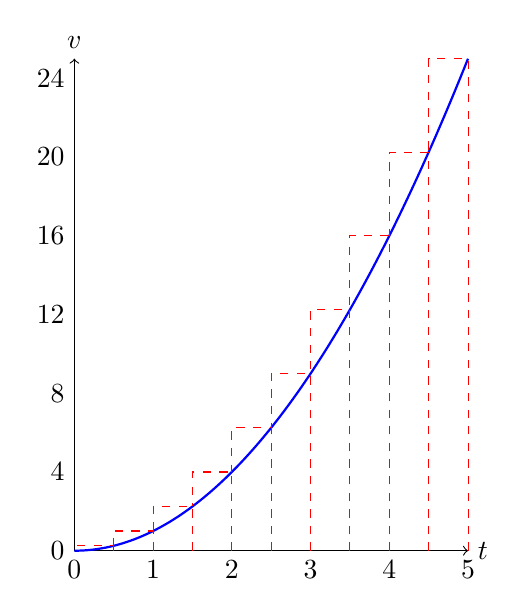
\begin{tikzpicture}[scale=0.5]
	\draw[->] (0,0) -- (10,0);
	\node[right] at (10,0) {$t$};
	\draw[->] (0,0) -- (0,12.5);
	\node[above] at (0,12.5) {$v$};
	\foreach \i in {0,...,5}{
		\node[below] at (2*\i,0) {$\i$};
	}
	\foreach \i in {0,4,...,24}{
		\node[left] at (0,0.5*\i) {$\i$};
	}
	
	\draw[blue,thick,domain=0:10,samples=100] plot (\x,{0.5*(0.5*\x)^2});
	
	\foreach \i in {1,...,10}{
		\draw[dashed,red] (\i,0) -- (\i,0.125*\i*\i) -- (\i-1,0.125*\i*\i) -- (\i-1,0.125*\i*\i-0.25*\i+0.125);
	}
	
\end{tikzpicture}
\end{center}




\clearpage










\textbf{Theory: The Trapezium Rule:}

\bigskip

When drawing a rectangle over a small interval to estimate the area under a curve, we have a choice: we can draw the rectangle up to the lowest point on the curve over that interval, or to the highest, or to any point in between. When defining the integral, it was convenient just to always draw it up to the value of the function at the right-hand endpoint of the interval, because we we take the limit, it won't matter. But when using only a finite number of rectangles to estimate the area, it seems clear that a good choice is to take the height of the rectangle to be halfway between the highest and lowest values of the function on that interval.

However, we might not know the highest and lowest values of the function on the interval; however, taking the height of the function at the left of the interval, the height of the function at the right, and going halfway between seems like a good compromise.

\begin{center}
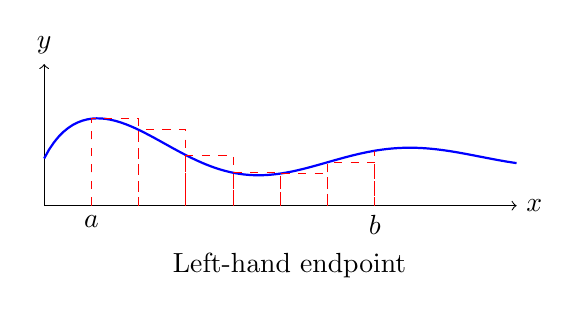
\begin{tikzpicture}[scale=0.6]
	\draw[->] (0,0) -- (10,0);
	\node[right] at (10,0) {$x$};
	\draw[->] (0,0) -- (0,3);
	\node[above] at (0,3) {$y$};
	
	\draw[blue,thick,domain=0:10,samples=100] plot (\x, { 1+ 2*sin(\x r)*(1-\x/(1+\x)) });
	\draw[red,dashed] (1,0) -- (1,{1+sin(1 r)});
	\draw[red,dashed] (7,0) -- (7,{1+0.25*sin(7 r)});
	\node[below] at (1,0) {$a$};
	\node[below] at (7,0) {$b$};
	
	\foreach \i in {1,2,...,6}{
		\draw[red,dashed] (\i,0) -- (\i, { 1+2*sin(\i r)*(1-\i/(1+\i)) }) -- ({\i+1}, { 1+2*sin(\i r)*(1-\i/(1+\i)) }) -- ({\i+1},0);
	}
	
	\node[below] at (current bounding box.south) {Left-hand endpoint};
\end{tikzpicture}
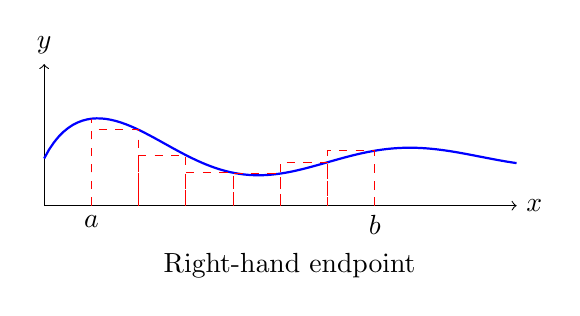
\begin{tikzpicture}[scale=0.6]
	\draw[->] (0,0) -- (10,0);
	\node[right] at (10,0) {$x$};
	\draw[->] (0,0) -- (0,3);
	\node[above] at (0,3) {$y$};
	
	\draw[blue,thick,domain=0:10,samples=100] plot (\x, { 1+ 2*sin(\x r)*(1-\x/(1+\x)) });
	\draw[red,dashed] (1,0) -- (1,{1+sin(1 r)});
	\draw[red,dashed] (7,0) -- (7,{1+0.25*sin(7 r)});
	\node[below] at (1,0) {$a$};
	\node[below] at (7,0) {$b$};
	
	\foreach \i in {1,2,...,6}{
		\draw[red,dashed] (\i,0) -- (\i, { 1+2*sin((\i+1) r)*(1-(\i+1)/(2+\i)) }) -- ({\i+1}, { 1+2*sin((\i+1) r)*(1-(\i+1)/(2+\i)) }) -- ({\i+1},0);
	}
	
	\node[below] at (current bounding box.south) {Right-hand endpoint};
\end{tikzpicture}

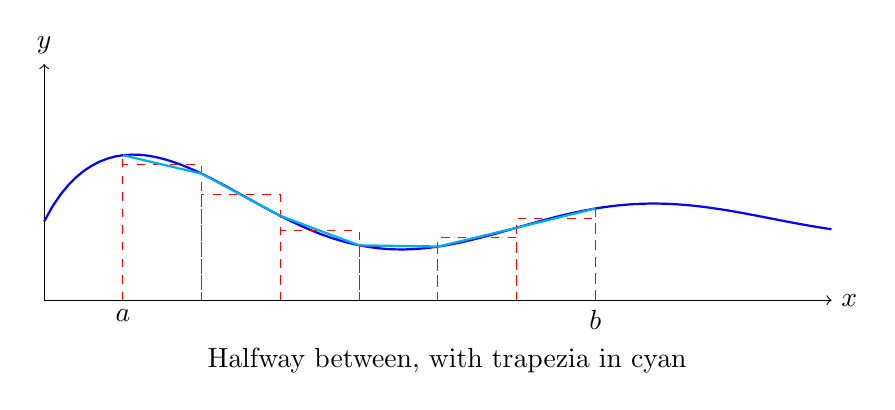
\begin{tikzpicture}[scale=1]
	\draw[->] (0,0) -- (10,0);
	\node[right] at (10,0) {$x$};
	\draw[->] (0,0) -- (0,3);
	\node[above] at (0,3) {$y$};
	
	\draw[blue,thick,domain=0:10,samples=100] plot (\x, { 1+ 2*sin(\x r)*(1-\x/(1+\x)) });
	\draw[red,dashed] (1,0) -- (1,{1+sin(1 r)});
	\draw[red,dashed] (7,0) -- (7,{1+0.25*sin(7 r)});
	\node[below] at (1,0) {$a$};
	\node[below] at (7,0) {$b$};
	
	\foreach \i in {1,2,...,6}{
		\draw[red,dashed] (\i,0) -- (\i, { 0.5*( 1+2*sin(\i r)*(1-\i/(1+\i)) ) + 0.5*( 1+2*sin((\i+1) r)*(1-(\i+1)/(2+\i))) }) -- ({\i+1}, { 0.5*( 1+2*sin(\i r)*(1-\i/(1+\i)) ) + 0.5*( 1+2*sin((\i+1) r)*(1-(\i+1)/(2+\i))) }) -- ({\i+1},0);
	}
	
	\foreach \i in {1,2,...,6}{
		\draw[thick,cyan] (\i, { 1+2*sin(\i r)*(1-\i/(1+\i)) }) -- ({\i+1}, { 1+2*sin((\i+1) r)*(1-(\i+1)/(2+\i)) });
	}
	
	\node[below] at (current bounding box.south) {Halfway between, with trapezia in cyan};
\end{tikzpicture}
\end{center}

So over each subinterval, from $x=a+\frac{k(b-a)}{n}$ to $x+\delta x=a+\frac{(k+1)(b-a)}{n}$, we should use $\frac{1}{2}(f(x)+f(x+\delta x))$ as the height of our rectangle. This is the same as the area of a trapezium with one leg of height $f(x)$ and the other of height $f(x+\delta x)$. Adding up the areas of these trapezia, and letting $h=\frac{b-a}{n}$, we have
\begin{align*}
	\int_a^b f(x)\diff x &\approx h\sum_{k=0}^n \frac{f(a+kh)+f(a+(k+1)h)}{2}\\
	&= \frac{h}{2}\left[f(a) + 2\left(\sum_{k=1}^{n-1} f(a+kh)\right) + f(b)\right]
\end{align*}




\clearpage





























\textbf{Practice:}\bigskip

The Trapezium rule, where $h=\frac{b-a}{n}$:
\begin{align*}
	\int_a^b f(x)\diff x &\approx \frac{h}{2}\left[f(a)+2\left(\sum_{k=1}^{n-1}f(a+kh)\right)+f(b)\right]\\
	&=\frac{h}{2}\left(f(a)+2f(a+h) + 2f(a+2h) + \hdots + 2f(a+(n-1)h) + f(b)\right).
\end{align*}



\begin{enumerate}
	\item Use the trapezium rule with $n=3$ to estimate the arc length of the curve $y=\sec(x)$ for $0\leq x\leq \frac{\pi}{4}$.
	\item In probability and statistics, the Standard Normal Distribution is of central importance. If a random variable $Z$ follows a Standard Normal Distribution, then the probability that a measured value of $Z$ is less than $z$ is given by the integral
		\[\frac{1}{\sqrt{2\pi}}\int_{-\infty}^z e^{-x^2/2}\diff x.\]
		Since $e^{-x^2/2}$ becomes very small as $x$ gets away from 0, we can take the integral from some moderately big negative number, instead of $-\infty$, without changing the answer much. Estimate the probability that a Standard Normal Variable is measured as having a value less than 0, by estimating
		\[\frac{1}{\sqrt{2\pi}}\int_{-3}^0 e^{-x^2/2}\diff x\]
		using the trapezium rule with $n=3$. Note: the correct value is 0.5, as the Standard Normal Distribution is symmetrical about $0$.
	\item We saw on an earlier sheet that
		\[\int_{-\infty}^\infty H(x)e^{-x}e^{-2\pi j fx}\diff x = \frac{1}{1+2\pi jf},\]
		where $H$ is the Heaviside function. This means that $\frac{1}{1+2\pi jf}$ is the Fourier transform of $H(x)e^{-x}$, as we shall see in our Fourier chapter. The inverse transform is given by
		\[\int_{-\infty}^\infty \frac{1}{1+2\pi j f}e^{2\pi j fx}\diff f,\]
		so this should give $H(x)e^{-x}$. With the tools we have covered, it is not possible for us to solve this integral analytically. However, for any fixed value of $x$, numerical methods (such as the trapezium rule) can be used to estimate the value of the inverse transform at $x$. In particular, since the inverse transform should be $H(x)e^{-x}$, it should give the values 0 at $x=-1$ and $e$ at $x=1$. Verify this by using the trapezium rule with $n=4$ to estimate the values of the inverse transform at these two points, choosing an appropriate value in place of $\infty$ in the limits of integration.
\end{enumerate}











\clearpage







{\bf Key Points to Remember:}

\vspace{5mm}

\begin{enumerate}
	\item Although some functions cannot be integrated analytically with the techniques we have developed (or, in some cases, with any known techniques!), they can be estimated numerically.
	\item A standard method for numerically estimating integrals is the \textbf{trapezium rule}, where the domain of integration is divided into small intervals, and the function approximated by a straight line over each interval, so the area becomes a sum of trapezia. With $n$ subdivisions, and $h=\frac{b-a}{n}$, this gives the formula
		\begin{align*}
			\int_a^b f(x)\diff x &\approx \frac{h}{2}\left[f(a)+2\left(\sum_{k=1}^{n-1}f(a+kh)\right)+f(b)\right]\\
			&=\frac{h}{2}\left(f(a)+2f(a+h) + 2f(a+2h) + \hdots + 2f(a+(n-1)h) + f(b)\right).
		\end{align*}
	\item If an integral is taken to infinity, we can replace infinity by a sufficiently large number for numerical approximation (how large is ``sufficiently large'' will depend on the function being integrated!).
	\item Other techniques for numerical integration exist; a common one is Simpson's Rule, which uses quadratics instead of straight lines to approximate the function over each subinterval, and gives more accurate estimates than the trapezium rule. Techniques such as the trapezium rule and Simpson's Rule are easy to implement on a computer, and many programs exist capable of estimating the vaue of an integral.
\end{enumerate}









\end{document}